\begin{frame}
	\frametitle{Project Background}
	Nuclear fusion -- the energy of the future!
    \vspace{10pt}
	\begin{itemize}
	    \item Must produce and contain an extremely hot and dense plasma
	    \begin{itemize}
		    \item Magnetic Confinement Fusion (MCF): toroidal circulation
		    \item Inertial Confinement Fusion (ICF): spherical compression
		\end{itemize}
		\vspace{10pt}
		\item Modern designs require enriched Hydrogen fuel of two varieties:
	    \begin{itemize}
		    \item Deuterium ($^2$H) -- abundant in naturally-sourced water
		    \item Tritium ($^3$H) -- extremely rare, but can be produced \textit{in-reactor}
		\end{itemize}
	\end{itemize}
	\vspace{10pt}
	\centering{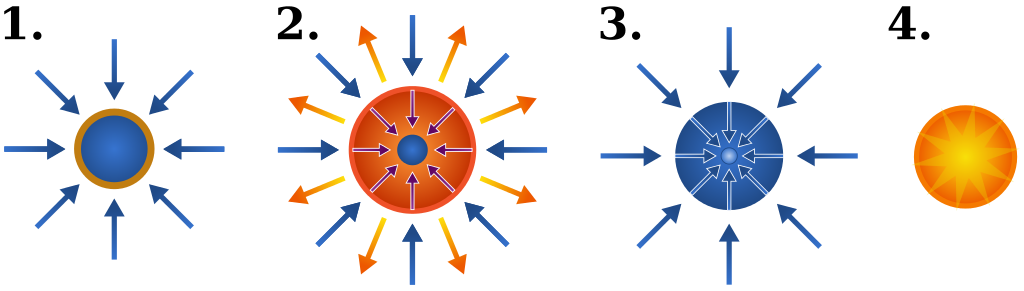
\includegraphics[height=3cm]{icf_diagram}}
\end{frame}

\begin{frame}
	\frametitle{Problem Description}
	Tritium breeding blankets convert neutron radiation from the fusion plasma into a steady supply of tritium fuel.
	\begin{align*}
		\isotope[1][0]{n} + \isotope[6][3]{Li} \rightarrow \isotope[3][1]{H} +
		\isotope[4][2]{He}
		\qquad\qquad
		\isotope[1][0]{n} + \isotope[7][3]{Li} \rightarrow \isotope[3][1]{H} +
		\isotope[4][2]{He} + \isotope[1][0]{n}
	\end{align*}
	However, the tritium breeding ratio (TBR) depends on numerous geometric and material parameters.\newline
	
	TBR evaluation \textit{Paramak} achieves very accurate results by OpenMC Monte Carlo neutronics simulation, but is computationally expensive.
	
	\vspace{15pt}
	
	\begin{center}
	    \textbf{Our Challenge:}
	\end{center}
	
	\begin{center}
	    \textbf{Produce a fast TBR function which strongly approximates Paramak, making use of the latest in surrogate modelling techniques.}
	\end{center}
\end{frame}

\begin{frame}
	\frametitle{Data Generation}
	We designed the Approximate TBR Evaluator (ATE) package to generate training and test datasets from Paramak.\newline
	 \begin{columns}[onlytextwidth,T]
      \column{\dimexpr\linewidth-6cm-5mm}
        
        UCL's Hypatia cluster provided the multithreading power for us to produce one million TBR samples, representing 27 days of runtime.\newline
        
        These runs included full evaluations on the 18 continuous and discrete parameters of Paramak, and "slice" evaluations with all discrete parameters frozen.

      \column{6cm}
      \vspace{0cm}
      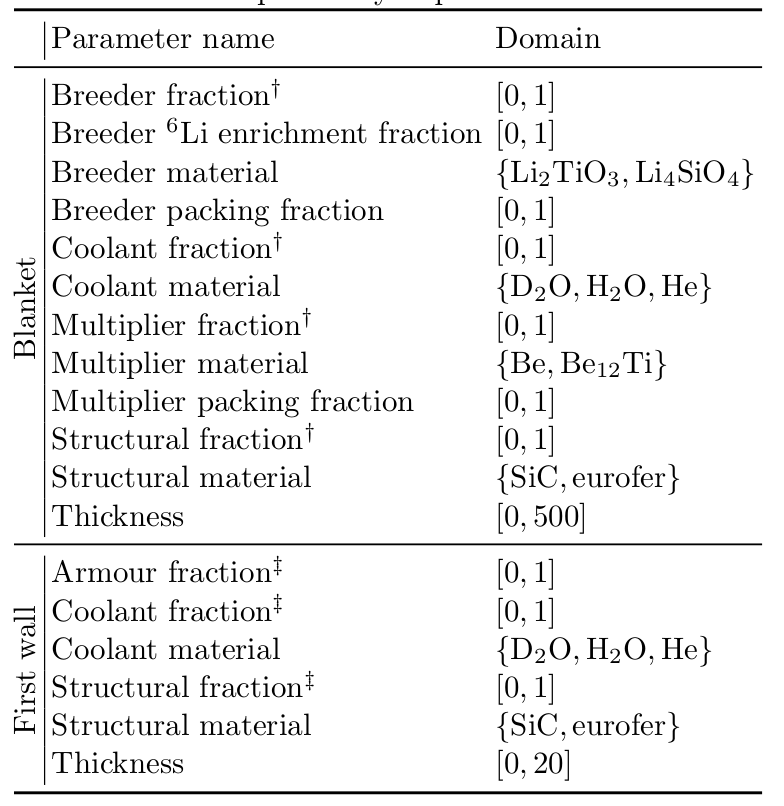
\includegraphics[trim={0 0 0 2mm},clip,width=6cm]{params}

    \end{columns}
\end{frame}

%\begin{frame}
%	\frametitle{Dimensionality Reduction}
%	\begin{itemize}
%		\item % TODO
%	\end{itemize}
%\end{frame}

\begin{frame}
	\frametitle{Methodology}
			Conventional regression task -- search for a cheap surrogate $\hat{f}(x)$ that
			minimizes dissimilarity with an expensive function $f(x)$:

			\begin{itemize}
				\item
					Regression performance: mean absolute error, $\sigma$ of
					error, $R^2$, $R^2_\text{adj.}$
				\item
					Computational complexity:
					training \& prediction time / sample.
			\end{itemize}

			2 approaches for surrogate training:
			\begin{enumerate}
				\item
					Decoupled -- trains models from previously sampled
					datapoints.
				\item
					Adaptive -- repeats sampling \& model training, increases
					sampling density in low-performance regions.
			\end{enumerate}
\end{frame}

